%%%%%%%%%%%%%%%%%%%%%%%%%%%%%%%%%%%%%%%%%%%%%%%%%%%%%%%%%%%%
% 2.7 DIOPHANTINE GEOMETRY
% The Composition of Advanced Mathematics
%%%%%%%%%%%%%%%%%%%%%%%%%%%%%%%%%%%%%%%%%%%%%%%%%%%%%%%%%%%%

\section{Diophantine Geometry}
\label{sec:diophantine-geometry}

\prerequisite{
Elementary Number Theory from \cref{sec:elementary-number-theory},
Diophantine Approximation from \cref{sec:diophantine-approximation}, and
basic polynomial algebra. Familiarity with fields, rings, and polynomial
equations from Chapter 1 is helpful. Algebraic geometry is developed
canonically in Chapter 3.
}

\learningobjectives{
By the end of this section, the reader should be able to:
\begin{itemize}
    \item explain the central viewpoint of Diophantine geometry;
    \item interpret integer and rational solutions as geometric points;
    \item distinguish affine and projective formulations of Diophantine equations;
    \item explain why homogenization introduces points at infinity;
    \item determine rational points on elementary curves;
    \item parameterize rational points on the unit circle;
    \item connect rational points on conics with Pythagorean triples;
    \item explain why the existence of one rational point can simplify a conic;
    \item distinguish curves according to genus at a conceptual level;
    \item explain why genus strongly influences rational-point behavior;
    \item recognize elliptic curves in Weierstrass form;
    \item describe the chord-and-tangent construction on an elliptic curve;
    \item explain how rational points on an elliptic curve form an abelian group;
    \item identify the point at infinity as the identity element;
    \item compute simple sums of rational points on elliptic curves;
    \item state the Mordell--Weil theorem;
    \item explain torsion and rank conceptually;
    \item define rational and integral points;
    \item understand the role of height functions;
    \item state Siegel's theorem conceptually;
    \item state Faltings's theorem conceptually;
    \item understand the significance of Fermat-type equations;
    \item explain the connection between Fermat's Last Theorem and algebraic curves;
    \item recognize local and global solvability as distinct questions;
    \item explain the local--global principle and its limitations;
    \item understand the role of reduction modulo primes;
    \item recognize the importance of rational points in arithmetic geometry;
    \item connect Diophantine geometry with algebraic geometry, algebraic number
    theory, topology, complex analysis, and cryptography.
\end{itemize}
}

%%%%%%%%%%%%%%%%%%%%%%%%%%%%%%%%%%%%%%%%%%%%%%%%%%%%%%%%%%%%
\subsection{From Equations to Geometry}
\label{subsec:diophantine-equations-to-geometry}
%%%%%%%%%%%%%%%%%%%%%%%%%%%%%%%%%%%%%%%%%%%%%%%%%%%%%%%%%%%%

A Diophantine equation asks for integer or rational solutions to a polynomial
equation.

For example,

\[ x^2+y^2=1 \]

can be viewed algebraically as an equation in two variables.

Geometrically, it defines a circle.

The rational solutions are therefore rational points lying on that circle.

This shift in viewpoint is the foundation of Diophantine geometry:

\[
\boxed{
\text{Diophantine equations}
\longleftrightarrow
\text{geometric objects with arithmetic points}.
}
\]

\begin{definitionbox}{Diophantine Geometry}
\emph{Diophantine geometry} studies integer, rational, and algebraic points
on geometric objects defined by polynomial equations.
\end{definitionbox}

Instead of asking only how to manipulate an equation, we study the geometry
of the entire solution set.

%%%%%%%%%%%%%%%%%%%%%%%%%%%%%%%%%%%%%%%%%%%%%%%%%%%%%%%%%%%%
\subsection{Arithmetic Points}
\label{subsec:arithmetic-points}
%%%%%%%%%%%%%%%%%%%%%%%%%%%%%%%%%%%%%%%%%%%%%%%%%%%%%%%%%%%%

Suppose

\[ F(x,y)=0 \]

is a polynomial equation.

A point

\[ (x,y)\in\R^2 \]

is a real point on the curve.

If

\[ x,y\in\Q, \]

then it is a \emph{rational point}.

If

\[ x,y\in\Z, \]

then it is an \emph{integral point}.

Thus we may study several sets:

\[
C(\R),\qquad C(\Q),\qquad C(\Z).
\]

The notation

\[ C(\Q) \]

is read ``the rational points of \(C\),'' while

\[ C(\Z) \]

is read ``the integral points of \(C\).''

Usually,

\[ C(\Z)\subseteq C(\Q)\subseteq C(\R). \]

%%%%%%%%%%%%%%%%%%%%%%%%%%%%%%%%%%%%%%%%%%%%%%%%%%%%%%%%%%%%
\subsection{A First Example}
\label{subsec:diophantine-geometry-first-example}
%%%%%%%%%%%%%%%%%%%%%%%%%%%%%%%%%%%%%%%%%%%%%%%%%%%%%%%%%%%%

Consider

\[ x^2+y^2=1. \]

Some rational points are

\[ (1,0),\qquad(0,1),\qquad\left(\frac35,\frac45\right). \]

But most real points are not rational.

Thus the geometric object is continuous, while the arithmetic subset may
have a highly structured distribution.

\begin{centereddiagram}
\begin{tikzpicture}[scale=1.7]
\draw[-{Latex[length=2.2mm]}] (-1.4,0)--(1.4,0) node[right] {\(x\)};
\draw[-{Latex[length=2.2mm]}] (0,-1.4)--(0,1.4) node[above] {\(y\)};
\draw[thick] (0,0) circle (1);

\foreach \x/\y in {1/0,-1/0,0/1,0/-1,0.6/0.8,0.6/-0.8,-0.6/0.8,-0.6/-0.8}{
    \fill (\x,\y) circle (1.8pt);
}
\node[right] at (0.6,0.8) {\scriptsize \(\left(\frac35,\frac45\right)\)};
\end{tikzpicture}
\end{centereddiagram}

%%%%%%%%%%%%%%%%%%%%%%%%%%%%%%%%%%%%%%%%%%%%%%%%%%%%%%%%%%%%
\subsection{Why Geometry Helps}
\label{subsec:why-geometry-helps-diophantine}
%%%%%%%%%%%%%%%%%%%%%%%%%%%%%%%%%%%%%%%%%%%%%%%%%%%%%%%%%%%%

The shape and structure of a polynomial equation can reveal arithmetic
information.

Geometry provides concepts such as:

\begin{itemize}
    \item dimension;
    \item singularity;
    \item intersection;
    \item tangent lines;
    \item genus;
    \item projective closure;
    \item morphisms;
    \item symmetry.
\end{itemize}

Arithmetic then asks which points have coordinates in

\[ \Z,\qquad\Q, \]

or more general number fields.

The interaction between these two perspectives is the central theme.

%%%%%%%%%%%%%%%%%%%%%%%%%%%%%%%%%%%%%%%%%%%%%%%%%%%%%%%%%%%%
\subsection{Affine Curves}
\label{subsec:affine-curves-diophantine}
%%%%%%%%%%%%%%%%%%%%%%%%%%%%%%%%%%%%%%%%%%%%%%%%%%%%%%%%%%%%

A polynomial equation

\[ F(x,y)=0 \]

defines an \emph{affine plane curve}.

Examples include

\[
x^2+y^2=1,
\qquad
y^2=x^3-x,
\qquad
x^3+y^3=1.
\]

The word \emph{affine} indicates that ordinary coordinates \(x\) and \(y\)
are being used.

A rational point is simply

\[ (x,y)\in\Q^2 \]

satisfying the equation.

%%%%%%%%%%%%%%%%%%%%%%%%%%%%%%%%%%%%%%%%%%%%%%%%%%%%%%%%%%%%
\subsection{Projective Coordinates}
\label{subsec:projective-coordinates-diophantine}
%%%%%%%%%%%%%%%%%%%%%%%%%%%%%%%%%%%%%%%%%%%%%%%%%%%%%%%%%%%%

Many arithmetic questions become cleaner after adding points at infinity.

Projective coordinates are written

\[ [X:Y:Z]. \]

The notation is read ``\(X\) colon \(Y\) colon \(Z\).''

Two triples represent the same projective point when

\[ [X:Y:Z]=[\lambda X:\lambda Y:\lambda Z] \]

for every nonzero scalar \(\lambda\).

Ordinary affine coordinates correspond to

\[ [x:y:1]. \]

Points satisfying

\[ Z=0 \]

are called \emph{points at infinity}.

%%%%%%%%%%%%%%%%%%%%%%%%%%%%%%%%%%%%%%%%%%%%%%%%%%%%%%%%%%%%
\subsection{Homogenization}
\label{subsec:homogenization-diophantine}
%%%%%%%%%%%%%%%%%%%%%%%%%%%%%%%%%%%%%%%%%%%%%%%%%%%%%%%%%%%%

To convert an affine polynomial equation into a projective equation, all
terms are given the same total degree.

For example,

\[ x^2+y^2=1 \]

becomes

\[ \boxed{X^2+Y^2=Z^2.} \]

Setting

\[ Z=1 \]

recovers the affine equation.

Setting

\[ Z=0 \]

reveals the points at infinity.

This process is called \emph{homogenization}.

%%%%%%%%%%%%%%%%%%%%%%%%%%%%%%%%%%%%%%%%%%%%%%%%%%%%%%%%%%%%
\subsection{Why Projective Geometry Matters}
\label{subsec:why-projective-diophantine}
%%%%%%%%%%%%%%%%%%%%%%%%%%%%%%%%%%%%%%%%%%%%%%%%%%%%%%%%%%%%

Projective geometry makes many algebraic curves complete by including their
behavior at infinity.

For example, two affine lines may appear parallel and never intersect.

In projective geometry, they meet at a point at infinity.

Likewise, elliptic curves acquire a distinguished point at infinity that
becomes the identity element of their group law.

Thus projective completion is not merely cosmetic.

It can reveal essential arithmetic structure.

%%%%%%%%%%%%%%%%%%%%%%%%%%%%%%%%%%%%%%%%%%%%%%%%%%%%%%%%%%%%
\subsection{Rational Points on Conics}
\label{subsec:rational-points-conics}
%%%%%%%%%%%%%%%%%%%%%%%%%%%%%%%%%%%%%%%%%%%%%%%%%%%%%%%%%%%%

A degree-two plane curve is called a \emph{conic}.

Examples include circles, ellipses, parabolas, and hyperbolas.

A remarkable fact is that once a nonsingular conic has one rational point,
its other rational points can often be parameterized using lines through
that point.

The unit circle gives the standard example.

%%%%%%%%%%%%%%%%%%%%%%%%%%%%%%%%%%%%%%%%%%%%%%%%%%%%%%%%%%%%
\subsection{Parameterizing the Unit Circle}
\label{subsec:parameterizing-unit-circle}
%%%%%%%%%%%%%%%%%%%%%%%%%%%%%%%%%%%%%%%%%%%%%%%%%%%%%%%%%%%%

Consider

\[ x^2+y^2=1. \]

The point

\[ (-1,0) \]

is rational.

Draw a line of rational slope \(t\) through this point:

\[ y=t(x+1). \]

Substitute into the circle equation:

\[ x^2+t^2(x+1)^2=1. \]

One solution is already

\[ x=-1. \]

The second intersection is

\[ x=\frac{1-t^2}{1+t^2}. \]

Substituting into the line gives

\[ y=\frac{2t}{1+t^2}. \]

Therefore

\[
\boxed{
x=\frac{1-t^2}{1+t^2},
\qquad
y=\frac{2t}{1+t^2}.
}
\]

If

\[ t\in\Q, \]

then both coordinates are rational.

%%%%%%%%%%%%%%%%%%%%%%%%%%%%%%%%%%%%%%%%%%%%%%%%%%%%%%%%%%%%
\subsection{Geometric Parameterization Visual}
\label{subsec:circle-parameterization-visual}
%%%%%%%%%%%%%%%%%%%%%%%%%%%%%%%%%%%%%%%%%%%%%%%%%%%%%%%%%%%%

\begin{centereddiagram}
\begin{tikzpicture}[scale=1.6]
\draw[-{Latex[length=2.2mm]}] (-1.5,0)--(1.5,0) node[right] {\(x\)};
\draw[-{Latex[length=2.2mm]}] (0,-1.35)--(0,1.35) node[above] {\(y\)};
\draw[thick] (0,0) circle (1);

\coordinate (A) at (-1,0);
\coordinate (B) at (0.6,0.8);

\draw[thick] (-1.25,-0.125)--(1.25,1.125);
\fill (A) circle (2pt);
\fill (B) circle (2pt);

\node[below left] at (A) {\((-1,0)\)};
\node[above right] at (B) {\(\left(\frac{1-t^2}{1+t^2},
\frac{2t}{1+t^2}\right)\)};
\node[above] at (0.05,0.58) {\(y=t(x+1)\)};
\end{tikzpicture}
\end{centereddiagram}

Every rational slope gives another rational point.

Conversely, every rational point on the circle other than \((-1,0)\)
determines a rational slope.

%%%%%%%%%%%%%%%%%%%%%%%%%%%%%%%%%%%%%%%%%%%%%%%%%%%%%%%%%%%%
\subsection{Worked Example: Rational Point from a Slope}
\label{subsec:worked-circle-rational-point}
%%%%%%%%%%%%%%%%%%%%%%%%%%%%%%%%%%%%%%%%%%%%%%%%%%%%%%%%%%%%

\begin{workedexamplebox}{Using \(t=\frac12\)}

Use

\[ t=\frac12 \]

to construct a rational point on

\[ x^2+y^2=1. \]

\begin{tabularx}{\textwidth}{@{}>{\raggedright\arraybackslash}p{0.43\textwidth}X@{}}
Use the \(x\)-parameterization. &
\(x=\dfrac{1-\frac14}{1+\frac14}\)\\
Simplify. & \(x=\frac35\)\\
Use the \(y\)-parameterization. &
\(y=\dfrac{1}{1+\frac14}\)\\
Simplify. & \(y=\frac45\)
\end{tabularx}

\begin{answerbox}
\[ \boxed{\left(\frac35,\frac45\right)} \]
\end{answerbox}
\end{workedexamplebox}

%%%%%%%%%%%%%%%%%%%%%%%%%%%%%%%%%%%%%%%%%%%%%%%%%%%%%%%%%%%%
\subsection{Pythagorean Triples Revisited}
\label{subsec:pythagorean-triples-geometry}
%%%%%%%%%%%%%%%%%%%%%%%%%%%%%%%%%%%%%%%%%%%%%%%%%%%%%%%%%%%%

A Pythagorean triple satisfies

\[ a^2+b^2=c^2. \]

If \(c\neq0\), divide by \(c^2\):

\[ \left(\frac ac\right)^2+\left(\frac bc\right)^2=1. \]

Thus Pythagorean triples correspond to rational points on the unit circle.

Let

\[ t=\frac mn. \]

Substituting into the rational parameterization gives

\[
x=\frac{n^2-m^2}{n^2+m^2},
\qquad
y=\frac{2mn}{n^2+m^2}.
\]

Hence

\[
\boxed{
a=n^2-m^2,\qquad
b=2mn,\qquad
c=n^2+m^2.
}
\]

The classical formula for Pythagorean triples is therefore a geometric
parameterization of rational points on a conic.

%%%%%%%%%%%%%%%%%%%%%%%%%%%%%%%%%%%%%%%%%%%%%%%%%%%%%%%%%%%%
\subsection{A General Conic Principle}
\label{subsec:general-conic-principle}
%%%%%%%%%%%%%%%%%%%%%%%%%%%%%%%%%%%%%%%%%%%%%%%%%%%%%%%%%%%%

The circle example illustrates a broader phenomenon.

\begin{importantbox}
A nonsingular conic defined over \(\Q\) that possesses one rational point can
be parameterized by rational functions.
\end{importantbox}

Geometrically, lines through a known rational point intersect the conic at
one additional point.

Algebraically, the second intersection has rational coordinates whenever the
line has rational coefficients.

Thus finding one rational point can unlock all rational points.

%%%%%%%%%%%%%%%%%%%%%%%%%%%%%%%%%%%%%%%%%%%%%%%%%%%%%%%%%%%%
\subsection{When Rational Points Do Not Exist}
\label{subsec:conics-no-rational-points}
%%%%%%%%%%%%%%%%%%%%%%%%%%%%%%%%%%%%%%%%%%%%%%%%%%%%%%%%%%%%

Not every curve has a rational point.

Consider

\[ x^2+y^2=3. \]

Real solutions clearly exist.

However, rational solvability requires additional arithmetic analysis.

This illustrates an important distinction:

\[
\boxed{
C(\R)\neq\varnothing
\quad\not\Longrightarrow\quad
C(\Q)\neq\varnothing.
}
\]

Real geometry alone does not determine rational solvability.

%%%%%%%%%%%%%%%%%%%%%%%%%%%%%%%%%%%%%%%%%%%%%%%%%%%%%%%%%%%%
\subsection{Local Solvability}
\label{subsec:local-solvability-diophantine}
%%%%%%%%%%%%%%%%%%%%%%%%%%%%%%%%%%%%%%%%%%%%%%%%%%%%%%%%%%%%

Before searching for rational solutions globally, one can test whether an
equation has solutions in simpler arithmetic settings.

For example, reduce an equation modulo a prime \(p\).

If an integer solution exists, then its coordinates must satisfy the reduced
equation modulo \(p\).

Therefore:

\[
\boxed{
\text{no solution modulo }p
\Longrightarrow
\text{no integer solution}.
}
\]

This gives a powerful obstruction.

%%%%%%%%%%%%%%%%%%%%%%%%%%%%%%%%%%%%%%%%%%%%%%%%%%%%%%%%%%%%
\subsection{Worked Example: Modular Obstruction}
\label{subsec:worked-modular-obstruction}
%%%%%%%%%%%%%%%%%%%%%%%%%%%%%%%%%%%%%%%%%%%%%%%%%%%%%%%%%%%%

\begin{workedexamplebox}{A Sum of Two Squares}

Show that

\[ x^2+y^2=3 \]

has no integer solutions.

\begin{tabularx}{\textwidth}{@{}>{\raggedright\arraybackslash}p{0.43\textwidth}X@{}}
Reduce modulo \(4\). & \(x^2+y^2\equiv3\pmod4\)\\
Squares modulo \(4\) are only. & \(0,1\)\\
Possible sums of two squares are. & \(0,1,2\pmod4\)\\
But \(3\) cannot occur. & Contradiction
\end{tabularx}

\begin{answerbox}
\[ \boxed{x^2+y^2=3\text{ has no integer solutions}.} \]
\end{answerbox}
\end{workedexamplebox}

%%%%%%%%%%%%%%%%%%%%%%%%%%%%%%%%%%%%%%%%%%%%%%%%%%%%%%%%%%%%
\subsection{The Local--Global Philosophy}
\label{subsec:local-global-philosophy}
%%%%%%%%%%%%%%%%%%%%%%%%%%%%%%%%%%%%%%%%%%%%%%%%%%%%%%%%%%%%

A central question is whether global rational solvability can be determined
from local solvability.

Very roughly, one asks:

\[
\boxed{
\text{solvable everywhere locally}
\stackrel{?}{\Longrightarrow}
\text{solvable globally}.
}
\]

The relevant local settings include:

\begin{itemize}
    \item the real numbers \(\R\);
    \item the \(p\)-adic numbers \(\Q_p\) for every prime \(p\).
\end{itemize}

The symbol

\[ \Q_p \]

is read ``the \(p\)-adic numbers.''

The \(p\)-adic numbers are developed more fully in Algebraic Number Theory.

%%%%%%%%%%%%%%%%%%%%%%%%%%%%%%%%%%%%%%%%%%%%%%%%%%%%%%%%%%%%
\subsection{The Hasse Principle}
\label{subsec:hasse-principle}
%%%%%%%%%%%%%%%%%%%%%%%%%%%%%%%%%%%%%%%%%%%%%%%%%%%%%%%%%%%%

\begin{definitionbox}{Hasse Principle}
An arithmetic variety is said to satisfy the \emph{Hasse principle} when
having points over \(\R\) and over every \(\Q_p\) implies that it has a
rational point over \(\Q\).
\end{definitionbox}

Many quadratic equations satisfy such a local--global principle.

But more complicated equations may fail it.

Thus local information is extremely useful but not universally sufficient.

%%%%%%%%%%%%%%%%%%%%%%%%%%%%%%%%%%%%%%%%%%%%%%%%%%%%%%%%%%%%
\subsection{Curves and Degree}
\label{subsec:curves-degree-diophantine}
%%%%%%%%%%%%%%%%%%%%%%%%%%%%%%%%%%%%%%%%%%%%%%%%%%%%%%%%%%%%

Polynomial degree gives an initial indication of geometric complexity.

Very roughly:

\[
\begin{array}{c|c|c}
\text{Degree} & \text{Typical smooth plane curve} & \text{Arithmetic behavior}\\
\hline
1 & \text{line} & \text{simple}\\
2 & \text{conic} & \text{often parameterizable}\\
3 & \text{cubic} & \text{elliptic behavior may appear}\\
\geq4 & \text{higher genus often appears} & \text{typically more rigid}
\end{array}
\]

Degree alone does not completely determine arithmetic behavior, but it is an
important first guide.

%%%%%%%%%%%%%%%%%%%%%%%%%%%%%%%%%%%%%%%%%%%%%%%%%%%%%%%%%%%%
\subsection{Genus}
\label{subsec:genus-diophantine}
%%%%%%%%%%%%%%%%%%%%%%%%%%%%%%%%%%%%%%%%%%%%%%%%%%%%%%%%%%%%

A fundamental geometric invariant of a smooth projective curve is its
\emph{genus}.

The genus is usually denoted

\[ g. \]

It is read ``genus \(g\).''

For complex curves, genus can be visualized topologically as the number of
handles of the corresponding surface.

\begin{centereddiagram}
\begin{tikzpicture}
\node[draw,rounded corners,minimum width=2.4cm,minimum height=1.2cm]
at (0,0) {\(g=0\)};
\node[draw,rounded corners,minimum width=2.4cm,minimum height=1.2cm]
at (3.3,0) {\(g=1\)};
\node[draw,rounded corners,minimum width=2.4cm,minimum height=1.2cm]
at (6.6,0) {\(g\geq2\)};

\draw[-{Latex[length=2.3mm]}] (1.25,0)--(2.05,0);
\draw[-{Latex[length=2.3mm]}] (4.55,0)--(5.35,0);

\node[below=4mm] at (0,0) {\scriptsize rational/conic type};
\node[below=4mm] at (3.3,0) {\scriptsize elliptic type};
\node[below=4mm] at (6.6,0) {\scriptsize higher-genus type};
\end{tikzpicture}
\end{centereddiagram}

%%%%%%%%%%%%%%%%%%%%%%%%%%%%%%%%%%%%%%%%%%%%%%%%%%%%%%%%%%%%
\subsection{Genus and Rational Points}
\label{subsec:genus-rational-points}
%%%%%%%%%%%%%%%%%%%%%%%%%%%%%%%%%%%%%%%%%%%%%%%%%%%%%%%%%%%%

The genus provides a remarkable first classification of rational-point
behavior.

Conceptually:

\[
\boxed{
\begin{array}{c|c}
g=0 & \text{zero or often infinitely many rational points}\\
g=1 & \text{rational points may form a finitely generated group}\\
g\geq2 & \text{only finitely many rational points}
\end{array}
}
\]

The last statement is a deep theorem and requires important qualifications:
the curve must be smooth, projective, and defined over a number field.

Nevertheless, genus is one of the strongest organizing principles in
Diophantine geometry.

%%%%%%%%%%%%%%%%%%%%%%%%%%%%%%%%%%%%%%%%%%%%%%%%%%%%%%%%%%%%
\subsection{Genus Zero}
\label{subsec:genus-zero-curves}
%%%%%%%%%%%%%%%%%%%%%%%%%%%%%%%%%%%%%%%%%%%%%%%%%%%%%%%%%%%%

Conics provide the standard genus-zero examples.

If a smooth projective genus-zero curve over \(\Q\) has a rational point,
then it behaves like the projective line

\[ \mathbb P^1. \]

Its rational points can then be parameterized.

Thus the unit-circle parameterization reflects the general geometry of
genus-zero curves.

%%%%%%%%%%%%%%%%%%%%%%%%%%%%%%%%%%%%%%%%%%%%%%%%%%%%%%%%%%%%
\subsection{Genus One}
\label{subsec:genus-one-curves}
%%%%%%%%%%%%%%%%%%%%%%%%%%%%%%%%%%%%%%%%%%%%%%%%%%%%%%%%%%%%

A smooth projective genus-one curve equipped with a chosen rational point
can be given the structure of an elliptic curve.

These curves are dramatically different from conics.

Their rational points need not admit a simple one-parameter
parameterization.

Instead, they possess an algebraic group structure.

%%%%%%%%%%%%%%%%%%%%%%%%%%%%%%%%%%%%%%%%%%%%%%%%%%%%%%%%%%%%
\subsection{Elliptic Curves}
\label{subsec:elliptic-curves-diophantine}
%%%%%%%%%%%%%%%%%%%%%%%%%%%%%%%%%%%%%%%%%%%%%%%%%%%%%%%%%%%%

Over a field of characteristic not \(2\) or \(3\), an elliptic curve can
often be written in short Weierstrass form:

\[ \boxed{E:y^2=x^3+Ax+B.} \]

The equation must be nonsingular.

For this form, nonsingularity is equivalent to

\[ 4A^3+27B^2\neq0. \]

The symbol

\[ E \]

is commonly used for an elliptic curve.

%%%%%%%%%%%%%%%%%%%%%%%%%%%%%%%%%%%%%%%%%%%%%%%%%%%%%%%%%%%%
\subsection{An Elliptic Curve Visual}
\label{subsec:elliptic-curve-visual}
%%%%%%%%%%%%%%%%%%%%%%%%%%%%%%%%%%%%%%%%%%%%%%%%%%%%%%%%%%%%

Consider

\[ E:y^2=x^3-x+1. \]

\begin{centereddiagram}
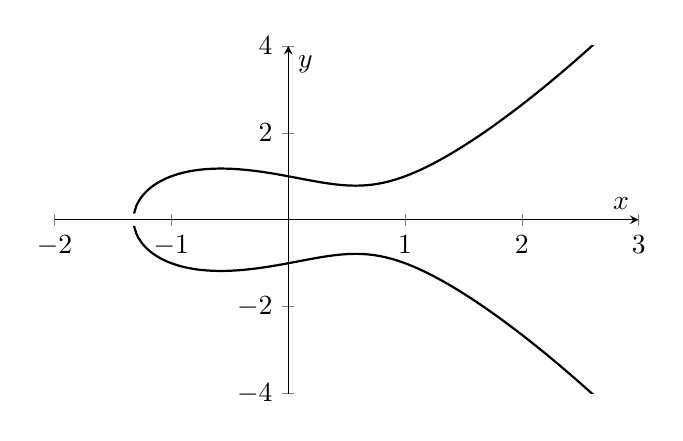
\begin{tikzpicture}
\begin{axis}[
    width=9cm,
    height=6cm,
    axis lines=middle,
    xmin=-2,xmax=3,
    ymin=-4,ymax=4,
    xlabel=\(x\),
    ylabel=\(y\),
    samples=220,
    domain=-1.32:3
]
\addplot[thick] {sqrt(x^3-x+1)};
\addplot[thick] {-sqrt(x^3-x+1)};
\end{axis}
\end{tikzpicture}
\end{centereddiagram}

Unlike a circle, an elliptic curve has a cubic shape.

Its geometry supports an unexpected arithmetic operation on points.

%%%%%%%%%%%%%%%%%%%%%%%%%%%%%%%%%%%%%%%%%%%%%%%%%%%%%%%%%%%%
\subsection{The Point at Infinity}
\label{subsec:elliptic-point-infinity}
%%%%%%%%%%%%%%%%%%%%%%%%%%%%%%%%%%%%%%%%%%%%%%%%%%%%%%%%%%%%

The projective form of

\[ y^2=x^3+Ax+B \]

is

\[ Y^2Z=X^3+AXZ^2+BZ^3. \]

Setting

\[ Z=0 \]

gives the unique projective point

\[ [0:1:0]. \]

This point is traditionally denoted

\[ \mathcal O. \]

The symbol is read ``script O'' or ``the point at infinity.''

It becomes the identity element of the elliptic-curve group.

%%%%%%%%%%%%%%%%%%%%%%%%%%%%%%%%%%%%%%%%%%%%%%%%%%%%%%%%%%%%
\subsection{Chord-and-Tangent Construction}
\label{subsec:elliptic-chord-tangent}
%%%%%%%%%%%%%%%%%%%%%%%%%%%%%%%%%%%%%%%%%%%%%%%%%%%%%%%%%%%%

Suppose

\[ P,Q\in E. \]

Draw the line through \(P\) and \(Q\).

A line intersects a cubic curve in three points when intersections are
counted appropriately.

Let the third intersection be \(R\).

Reflect \(R\) across the \(x\)-axis.

The reflected point is defined to be

\[ P+Q. \]

\begin{centereddiagram}
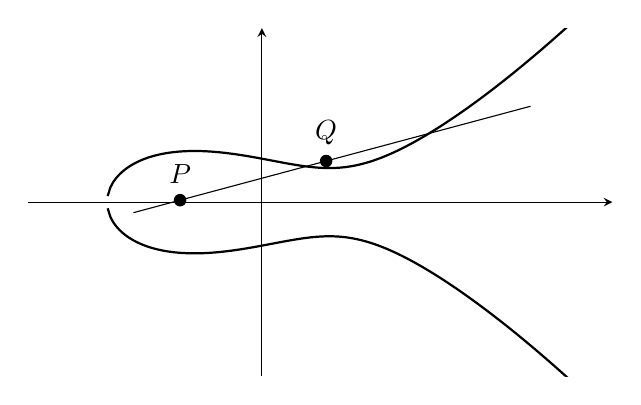
\begin{tikzpicture}
\begin{axis}[
    width=9cm,
    height=6cm,
    axis lines=middle,
    xmin=-2,xmax=3,
    ymin=-4,ymax=4,
    samples=180,
    domain=-1.32:3,
    xtick=\empty,
    ytick=\empty
]
\addplot[thick] {sqrt(x^3-x+1)};
\addplot[thick] {-sqrt(x^3-x+1)};
\addplot[domain=-1.1:2.3] {0.72*x+0.55};

\node[circle,fill,inner sep=1.6pt,label=above:\(P\)]
at (axis cs:-0.7,0.046) {};
\node[circle,fill,inner sep=1.6pt,label=above:\(Q\)]
at (axis cs:0.55,0.946) {};
\end{axis}
\end{tikzpicture}
\end{centereddiagram}

The diagram is schematic; the essential idea is the
line--third-intersection--reflection process.

%%%%%%%%%%%%%%%%%%%%%%%%%%%%%%%%%%%%%%%%%%%%%%%%%%%%%%%%%%%%
\subsection{Adding Distinct Points}
\label{subsec:elliptic-add-distinct-points}
%%%%%%%%%%%%%%%%%%%%%%%%%%%%%%%%%%%%%%%%%%%%%%%%%%%%%%%%%%%%

Let

\[ P=(x_1,y_1),\qquad Q=(x_2,y_2) \]

be distinct points with

\[ x_1\neq x_2. \]

The slope of the line through them is

\[ m=\frac{y_2-y_1}{x_2-x_1}. \]

Then

\[ \boxed{x_3=m^2-x_1-x_2} \]

and

\[ \boxed{y_3=m(x_1-x_3)-y_1}. \]

The sum is

\[ P+Q=(x_3,y_3). \]

If the original points have rational coordinates, these formulas show that
their sum also has rational coordinates.

%%%%%%%%%%%%%%%%%%%%%%%%%%%%%%%%%%%%%%%%%%%%%%%%%%%%%%%%%%%%
\subsection{Doubling a Point}
\label{subsec:elliptic-point-doubling}
%%%%%%%%%%%%%%%%%%%%%%%%%%%%%%%%%%%%%%%%%%%%%%%%%%%%%%%%%%%%

When

\[ P=Q, \]

the secant line becomes the tangent line.

For

\[ E:y^2=x^3+Ax+B \]

and

\[ P=(x_1,y_1),\qquad y_1\neq0, \]

the tangent slope is

\[ m=\frac{3x_1^2+A}{2y_1}. \]

Then

\[ x_3=m^2-2x_1 \]

and

\[ y_3=m(x_1-x_3)-y_1. \]

The resulting point is

\[ 2P=P+P. \]

%%%%%%%%%%%%%%%%%%%%%%%%%%%%%%%%%%%%%%%%%%%%%%%%%%%%%%%%%%%%
\subsection{Inverse Points}
\label{subsec:elliptic-inverse-points}
%%%%%%%%%%%%%%%%%%%%%%%%%%%%%%%%%%%%%%%%%%%%%%%%%%%%%%%%%%%%

If

\[ P=(x,y), \]

then its inverse is

\[ \boxed{-P=(x,-y).} \]

Geometrically, \(P\) and \(-P\) are reflections across the \(x\)-axis.

The vertical line through them meets the curve at the point at infinity.

Therefore

\[ \boxed{P+(-P)=\mathcal O.} \]

%%%%%%%%%%%%%%%%%%%%%%%%%%%%%%%%%%%%%%%%%%%%%%%%%%%%%%%%%%%%
\subsection{Elliptic-Curve Group}
\label{subsec:elliptic-curve-group}
%%%%%%%%%%%%%%%%%%%%%%%%%%%%%%%%%%%%%%%%%%%%%%%%%%%%%%%%%%%%

The rational points together with the point at infinity form an abelian
group:

\[ \boxed{E(\Q).} \]

The operation satisfies:

\begin{itemize}
    \item closure;
    \item associativity;
    \item identity \(\mathcal O\);
    \item inverses;
    \item commutativity.
\end{itemize}

Associativity is the difficult property to prove directly from the geometric
construction.

The full proof belongs naturally to algebraic geometry.

%%%%%%%%%%%%%%%%%%%%%%%%%%%%%%%%%%%%%%%%%%%%%%%%%%%%%%%%%%%%
\subsection{Worked Example: Adding Rational Points}
\label{subsec:worked-elliptic-addition}
%%%%%%%%%%%%%%%%%%%%%%%%%%%%%%%%%%%%%%%%%%%%%%%%%%%%%%%%%%%%

Consider

\[ E:y^2=x^3-x+1. \]

The points

\[ P=(0,1),\qquad Q=(1,1) \]

lie on \(E\).

\begin{workedexamplebox}{Adding \(P=(0,1)\) and \(Q=(1,1)\)}

\begin{tabularx}{\textwidth}{@{}>{\raggedright\arraybackslash}p{0.43\textwidth}X@{}}
Compute the slope. &
\(m=\dfrac{1-1}{1-0}=0\)\\
Compute the new \(x\)-coordinate. &
\(x_3=0^2-0-1=-1\)\\
Compute the new \(y\)-coordinate. &
\(y_3=0(0-(-1))-1=-1\)\\
Therefore. &
\(P+Q=(-1,-1)\)
\end{tabularx}

\begin{answerbox}
\[ \boxed{(0,1)+(1,1)=(-1,-1).} \]
\end{answerbox}
\end{workedexamplebox}

Indeed,

\[ (-1)^2=(-1)^3-(-1)+1=1. \]

%%%%%%%%%%%%%%%%%%%%%%%%%%%%%%%%%%%%%%%%%%%%%%%%%%%%%%%%%%%%
\subsection{Worked Example: Doubling a Point}
\label{subsec:worked-elliptic-doubling}
%%%%%%%%%%%%%%%%%%%%%%%%%%%%%%%%%%%%%%%%%%%%%%%%%%%%%%%%%%%%

Again consider

\[ E:y^2=x^3-x+1 \]

and

\[ P=(0,1). \]

\begin{workedexamplebox}{Computing \(2P\)}

\begin{tabularx}{\textwidth}{@{}>{\raggedright\arraybackslash}p{0.43\textwidth}X@{}}
Here \(A=-1\). Compute the tangent slope. &
\(m=\dfrac{3(0)^2-1}{2(1)}=-\frac12\)\\
Compute the new \(x\)-coordinate. &
\(x_3=\frac14-0=\frac14\)\\
Compute the new \(y\)-coordinate. &
\(y_3=-\frac12(0-\frac14)-1=-\frac78\)
\end{tabularx}

\begin{answerbox}
\[ \boxed{2P=\left(\frac14,-\frac78\right).} \]
\end{answerbox}
\end{workedexamplebox}

%%%%%%%%%%%%%%%%%%%%%%%%%%%%%%%%%%%%%%%%%%%%%%%%%%%%%%%%%%%%
\subsection{Repeated Addition}
\label{subsec:elliptic-repeated-addition}
%%%%%%%%%%%%%%%%%%%%%%%%%%%%%%%%%%%%%%%%%%%%%%%%%%%%%%%%%%%%

Once a rational point \(P\) is known, one may form

\[ P,\quad2P,\quad3P,\quad4P,\ldots \]

using the group law.

If these points never repeat, then the curve has infinitely many rational
points.

Thus a single rational point of infinite order can generate infinitely many
others.

This is fundamentally different from the rational parameterization of a
conic.

%%%%%%%%%%%%%%%%%%%%%%%%%%%%%%%%%%%%%%%%%%%%%%%%%%%%%%%%%%%%
\subsection{Torsion Points}
\label{subsec:elliptic-torsion-points}
%%%%%%%%%%%%%%%%%%%%%%%%%%%%%%%%%%%%%%%%%%%%%%%%%%%%%%%%%%%%

\begin{definitionbox}{Torsion Point}
A point \(P\in E(\Q)\) is a \emph{torsion point} if there exists an integer
\(n\geq1\) such that

\[ \boxed{nP=\mathcal O.} \]
\end{definitionbox}

The smallest such positive integer \(n\) is the order of \(P\).

The set of rational torsion points is denoted

\[ E(\Q)_{\mathrm{tors}}. \]

It is read ``the torsion subgroup of \(E\) over the rationals.''

%%%%%%%%%%%%%%%%%%%%%%%%%%%%%%%%%%%%%%%%%%%%%%%%%%%%%%%%%%%%
\subsection{Points of Infinite Order}
\label{subsec:elliptic-infinite-order}
%%%%%%%%%%%%%%%%%%%%%%%%%%%%%%%%%%%%%%%%%%%%%%%%%%%%%%%%%%%%

If no positive multiple of \(P\) equals

\[ \mathcal O, \]

then \(P\) has \emph{infinite order}.

Such a point generates infinitely many rational points:

\[ \ldots,-2P,-P,\mathcal O,P,2P,3P,\ldots \]

Therefore the existence of a rational point of infinite order implies that

\[ E(\Q) \]

is infinite.

%%%%%%%%%%%%%%%%%%%%%%%%%%%%%%%%%%%%%%%%%%%%%%%%%%%%%%%%%%%%
\subsection{Mordell--Weil Theorem}
\label{subsec:mordell-weil-theorem}
%%%%%%%%%%%%%%%%%%%%%%%%%%%%%%%%%%%%%%%%%%%%%%%%%%%%%%%%%%%%

The rational points are nevertheless controlled by finitely many generators.

\begin{theorem}[Mordell--Weil]
Let \(E\) be an elliptic curve over \(\Q\). Then the abelian group

\[ E(\Q) \]

is finitely generated.
\end{theorem}

Therefore

\[ \boxed{E(\Q)\cong E(\Q)_{\mathrm{tors}}\oplus\Z^r} \]

for some nonnegative integer \(r\).

The integer

\[ r \]

is called the \emph{rank} of the elliptic curve.

%%%%%%%%%%%%%%%%%%%%%%%%%%%%%%%%%%%%%%%%%%%%%%%%%%%%%%%%%%%%
\subsection{Rank}
\label{subsec:elliptic-curve-rank}
%%%%%%%%%%%%%%%%%%%%%%%%%%%%%%%%%%%%%%%%%%%%%%%%%%%%%%%%%%%%

The rank measures the number of independent infinite-order generators.

Conceptually:

\[
\begin{array}{c|c}
r=0 & E(\Q)\text{ is finite}\\
r=1 & \text{one independent infinite-order direction}\\
r=2 & \text{two independent infinite-order directions}\\
\vdots & \vdots
\end{array}
\]

Determining the rank of a specific elliptic curve can be difficult.

The study of ranks is a major part of modern arithmetic geometry.

%%%%%%%%%%%%%%%%%%%%%%%%%%%%%%%%%%%%%%%%%%%%%%%%%%%%%%%%%%%%
\subsection{The Structure of \(E(\Q)\)}
\label{subsec:structure-rational-elliptic-points}
%%%%%%%%%%%%%%%%%%%%%%%%%%%%%%%%%%%%%%%%%%%%%%%%%%%%%%%%%%%%

The Mordell--Weil theorem gives the conceptual structure

\[
\boxed{
\text{rational points}
=
\text{finite torsion}
+
\text{finitely many infinite-order generators}.
}
\]

Thus an elliptic curve may have infinitely many rational points, but those
points are generated from finite arithmetic data.

This is one of the fundamental contrasts between genus \(1\) and genus \(0\).

%%%%%%%%%%%%%%%%%%%%%%%%%%%%%%%%%%%%%%%%%%%%%%%%%%%%%%%%%%%%
\subsection{Integral Points on Elliptic Curves}
\label{subsec:integral-points-elliptic}
%%%%%%%%%%%%%%%%%%%%%%%%%%%%%%%%%%%%%%%%%%%%%%%%%%%%%%%%%%%%

Even when

\[ E(\Q) \]

is infinite, the set of integral points

\[ E(\Z) \]

can be finite.

For example, repeated elliptic-curve addition often introduces larger and
larger denominators.

Thus rational abundance does not imply integral abundance.

This distinction is central in Diophantine equations.

%%%%%%%%%%%%%%%%%%%%%%%%%%%%%%%%%%%%%%%%%%%%%%%%%%%%%%%%%%%%
\subsection{Siegel's Theorem}
\label{subsec:siegel-theorem}
%%%%%%%%%%%%%%%%%%%%%%%%%%%%%%%%%%%%%%%%%%%%%%%%%%%%%%%%%%%%

A deep theorem gives broad finiteness results for integral points.

\begin{theorem}[Siegel]
Under standard hypotheses, an affine algebraic curve of genus at least \(1\)
has only finitely many integral points.
\end{theorem}

The precise theorem is formulated using number fields, \(S\)-integers, and
the geometry of the points removed from the projective curve.

The conceptual message is:

\[
\boxed{
\text{positive-genus curves typically have only finitely many integral points}.
}
\]

%%%%%%%%%%%%%%%%%%%%%%%%%%%%%%%%%%%%%%%%%%%%%%%%%%%%%%%%%%%%
\subsection{Higher-Genus Curves}
\label{subsec:higher-genus-curves}
%%%%%%%%%%%%%%%%%%%%%%%%%%%%%%%%%%%%%%%%%%%%%%%%%%%%%%%%%%%%

Curves of genus

\[ g\geq2 \]

are arithmetically more rigid than elliptic curves.

For a long time, it was conjectured that such curves should have only
finitely many rational points.

This was known as the Mordell conjecture.

%%%%%%%%%%%%%%%%%%%%%%%%%%%%%%%%%%%%%%%%%%%%%%%%%%%%%%%%%%%%
\subsection{Faltings's Theorem}
\label{subsec:faltings-theorem}
%%%%%%%%%%%%%%%%%%%%%%%%%%%%%%%%%%%%%%%%%%%%%%%%%%%%%%%%%%%%

\begin{theorem}[Faltings]
Let \(C\) be a smooth projective curve of genus

\[ g\geq2 \]

defined over a number field \(K\).

Then

\[ \boxed{C(K)\text{ is finite}.} \]
\end{theorem}

In particular, for a curve defined over \(\Q\),

\[ \boxed{C(\Q)\text{ is finite}.} \]

This theorem proved the Mordell conjecture.

%%%%%%%%%%%%%%%%%%%%%%%%%%%%%%%%%%%%%%%%%%%%%%%%%%%%%%%%%%%%
\subsection{The Genus Trichotomy}
\label{subsec:genus-trichotomy}
%%%%%%%%%%%%%%%%%%%%%%%%%%%%%%%%%%%%%%%%%%%%%%%%%%%%%%%%%%%%

The preceding results suggest a fundamental arithmetic classification:

\[
\boxed{
\begin{array}{c|c|c}
\text{Genus} & \text{Typical structure} & \text{Rational points}\\
\hline
0 & \text{rational curves} & \text{none or parameterizable}\\
1 & \text{elliptic curves} & \text{finitely generated group}\\
\geq2 & \text{higher-genus curves} & \text{finite}
\end{array}
}
\]

This table is a guiding principle rather than a substitute for the precise
hypotheses of the underlying theorems.

%%%%%%%%%%%%%%%%%%%%%%%%%%%%%%%%%%%%%%%%%%%%%%%%%%%%%%%%%%%%
\subsection{Height}
\label{subsec:height-diophantine-geometry}
%%%%%%%%%%%%%%%%%%%%%%%%%%%%%%%%%%%%%%%%%%%%%%%%%%%%%%%%%%%%

To study rational points quantitatively, we need a measure of arithmetic
size.

Suppose

\[ x=\frac ab \]

is written in lowest terms.

A simple height is

\[ H(x)=\max\{|a|,|b|\}. \]

The quantity

\[ H(x) \]

is read ``the height of \(x\).''

A logarithmic version is

\[ h(x)=\log H(x). \]

Height functions generalize this idea to projective points and algebraic
varieties.

%%%%%%%%%%%%%%%%%%%%%%%%%%%%%%%%%%%%%%%%%%%%%%%%%%%%%%%%%%%%
\subsection{Height of a Projective Point}
\label{subsec:projective-height}
%%%%%%%%%%%%%%%%%%%%%%%%%%%%%%%%%%%%%%%%%%%%%%%%%%%%%%%%%%%%

Let

\[ P=[X_0:X_1:\cdots:X_n] \]

be a rational projective point represented by coprime integers.

A basic projective height is

\[ \boxed{H(P)=\max\{|X_0|,\ldots,|X_n|\}.} \]

Height allows rational points to be ordered by arithmetic complexity.

One can then ask:

\begin{center}
How many rational points of height at most \(B\) lie on a variety?
\end{center}

This question leads to deep counting problems in arithmetic geometry.

%%%%%%%%%%%%%%%%%%%%%%%%%%%%%%%%%%%%%%%%%%%%%%%%%%%%%%%%%%%%
\subsection{Northcott-Type Finiteness}
\label{subsec:northcott-finiteness}
%%%%%%%%%%%%%%%%%%%%%%%%%%%%%%%%%%%%%%%%%%%%%%%%%%%%%%%%%%%%

Height behaves like a notion of arithmetic size.

For rational numbers, only finitely many reduced fractions satisfy

\[ H\left(\frac ab\right)\leq B. \]

More generally, bounded degree together with bounded height gives a finite
set of algebraic numbers.

This finiteness principle is one reason height functions are so powerful.

%%%%%%%%%%%%%%%%%%%%%%%%%%%%%%%%%%%%%%%%%%%%%%%%%%%%%%%%%%%%
\subsection{Canonical Height on Elliptic Curves}
\label{subsec:canonical-height-elliptic}
%%%%%%%%%%%%%%%%%%%%%%%%%%%%%%%%%%%%%%%%%%%%%%%%%%%%%%%%%%%%

Elliptic curves possess a refined height called the \emph{canonical height},
usually written

\[ \hat h(P). \]

The symbol

\[ \hat h \]

is read ``h hat.''

It interacts naturally with the group law:

\[ \boxed{\hat h(nP)=n^2\hat h(P).} \]

This quadratic growth makes canonical height extremely useful for studying
the Mordell--Weil group.

%%%%%%%%%%%%%%%%%%%%%%%%%%%%%%%%%%%%%%%%%%%%%%%%%%%%%%%%%%%%
\subsection{Reduction Modulo a Prime}
\label{subsec:reduction-mod-p-curves}
%%%%%%%%%%%%%%%%%%%%%%%%%%%%%%%%%%%%%%%%%%%%%%%%%%%%%%%%%%%%

Suppose a curve is defined by equations with integer coefficients.

Reducing those coefficients modulo a prime \(p\) produces a curve over the
finite field

\[ \F_p. \]

Rational or integral points can then be compared with points on the reduced
curve.

For elliptic curves, one studies

\[ E(\F_p). \]

The notation is read ``the points of \(E\) over the finite field with
\(p\) elements.''

%%%%%%%%%%%%%%%%%%%%%%%%%%%%%%%%%%%%%%%%%%%%%%%%%%%%%%%%%%%%
\subsection{Why Reduction Helps}
\label{subsec:why-reduction-helps}
%%%%%%%%%%%%%%%%%%%%%%%%%%%%%%%%%%%%%%%%%%%%%%%%%%%%%%%%%%%%

Reduction modulo primes can provide:

\begin{itemize}
    \item obstructions to integer solutions;
    \item information about torsion points;
    \item finite approximations to arithmetic structure;
    \item point counts over finite fields;
    \item data related to \(L\)-functions;
    \item computational tools for elliptic curves.
\end{itemize}

Thus finite-field arithmetic can reveal information about rational points
over \(\Q\).

%%%%%%%%%%%%%%%%%%%%%%%%%%%%%%%%%%%%%%%%%%%%%%%%%%%%%%%%%%%%
\subsection{Counting Points Modulo \(p\)}
\label{subsec:counting-points-mod-p}
%%%%%%%%%%%%%%%%%%%%%%%%%%%%%%%%%%%%%%%%%%%%%%%%%%%%%%%%%%%%

For an elliptic curve \(E\), define

\[ \#E(\F_p) \]

to be the number of points on the reduced curve over \(\F_p\), including the
point at infinity.

One writes

\[ \boxed{\#E(\F_p)=p+1-a_p.} \]

The quantity

\[ a_p \]

measures the deviation from \(p+1\).

These numbers become coefficients in the \(L\)-function of the elliptic
curve.

%%%%%%%%%%%%%%%%%%%%%%%%%%%%%%%%%%%%%%%%%%%%%%%%%%%%%%%%%%%%
\subsection{Hasse's Bound}
\label{subsec:hasse-bound-elliptic}
%%%%%%%%%%%%%%%%%%%%%%%%%%%%%%%%%%%%%%%%%%%%%%%%%%%%%%%%%%%%

\begin{theorem}[Hasse]
For an elliptic curve with good reduction modulo \(p\),

\[ \boxed{|a_p|\leq2\sqrt p.} \]
\end{theorem}

Equivalently,

\[ \boxed{|\#E(\F_p)-(p+1)|\leq2\sqrt p.} \]

Thus the number of points on an elliptic curve over a finite field is close
to \(p+1\).

%%%%%%%%%%%%%%%%%%%%%%%%%%%%%%%%%%%%%%%%%%%%%%%%%%%%%%%%%%%%
\subsection{Fermat Curves}
\label{subsec:fermat-curves}
%%%%%%%%%%%%%%%%%%%%%%%%%%%%%%%%%%%%%%%%%%%%%%%%%%%%%%%%%%%%

Fermat's equation

\[ x^n+y^n=z^n \]

can be converted, when \(z\neq0\), into

\[ X^n+Y^n=1 \]

by setting

\[ X=\frac{x}{z},\qquad Y=\frac{y}{z}. \]

Thus Fermat's Last Theorem can be interpreted as a statement about rational
points on the Fermat curve

\[ \boxed{X^n+Y^n=1.} \]

For

\[ n\geq3, \]

the nontrivial rational points are severely restricted.

%%%%%%%%%%%%%%%%%%%%%%%%%%%%%%%%%%%%%%%%%%%%%%%%%%%%%%%%%%%%
\subsection{Genus of Fermat Curves}
\label{subsec:fermat-curve-genus}
%%%%%%%%%%%%%%%%%%%%%%%%%%%%%%%%%%%%%%%%%%%%%%%%%%%%%%%%%%%%

The smooth projective Fermat curve

\[ X^n+Y^n=Z^n \]

has genus

\[ \boxed{g=\frac{(n-1)(n-2)}2.} \]

Thus:

\[
\begin{array}{c|c}
n & g\\
\hline
2 & 0\\
3 & 1\\
4 & 3\\
5 & 6
\end{array}
\]

The arithmetic difficulty grows dramatically as the geometry becomes more
complicated.

%%%%%%%%%%%%%%%%%%%%%%%%%%%%%%%%%%%%%%%%%%%%%%%%%%%%%%%%%%%%
\subsection{Fermat's Last Theorem}
\label{subsec:fermat-last-theorem-geometry}
%%%%%%%%%%%%%%%%%%%%%%%%%%%%%%%%%%%%%%%%%%%%%%%%%%%%%%%%%%%%

\begin{theorem}[Fermat's Last Theorem]
For every integer

\[ n>2, \]

there are no positive integers \(x,y,z\) satisfying

\[ \boxed{x^n+y^n=z^n.} \]
\end{theorem}

The modern proof does not simply solve each Fermat curve directly.

Instead, it connects hypothetical solutions to elliptic curves and modular
forms.

This is a striking example of the philosophy of modern number theory:

\[
\boxed{
\text{an arithmetic equation may be solved by studying a different
geometric object associated with it}.
}
\]

%%%%%%%%%%%%%%%%%%%%%%%%%%%%%%%%%%%%%%%%%%%%%%%%%%%%%%%%%%%%
\subsection{The Frey Curve Idea}
\label{subsec:frey-curve-idea}
%%%%%%%%%%%%%%%%%%%%%%%%%%%%%%%%%%%%%%%%%%%%%%%%%%%%%%%%%%%%

Suppose hypothetically that

\[ a^n+b^n=c^n \]

had a nontrivial solution for suitable exponent \(n\).

One can associate an elliptic curve of the general form

\[ y^2=x(x-a^n)(x+b^n). \]

This is called a \emph{Frey curve}.

The arithmetic properties of this elliptic curve would be extraordinarily
restrictive.

The contradiction ultimately arises from the relationship between elliptic
curves and modular forms.

The full proof lies far beyond this introductory section.

%%%%%%%%%%%%%%%%%%%%%%%%%%%%%%%%%%%%%%%%%%%%%%%%%%%%%%%%%%%%
\subsection{Modularity}
\label{subsec:elliptic-modularity-preview}
%%%%%%%%%%%%%%%%%%%%%%%%%%%%%%%%%%%%%%%%%%%%%%%%%%%%%%%%%%%%

A deep theorem states that elliptic curves over \(\Q\) are modular.

Very roughly, this means that an elliptic curve can be associated with a
modular form whose arithmetic data matches that of the curve.

Schematically,

\[
\boxed{
\text{elliptic curve}
\longleftrightarrow
\text{modular form}.
}
\]

This bridge connects geometry, algebra, analysis, and number theory.

It played a central role in the proof of Fermat's Last Theorem.

%%%%%%%%%%%%%%%%%%%%%%%%%%%%%%%%%%%%%%%%%%%%%%%%%%%%%%%%%%%%
\subsection{Elliptic-Curve \(L\)-Functions}
\label{subsec:elliptic-l-functions}
%%%%%%%%%%%%%%%%%%%%%%%%%%%%%%%%%%%%%%%%%%%%%%%%%%%%%%%%%%%%

The point-counting quantities

\[ a_p=p+1-\#E(\F_p) \]

can be assembled into an Euler product defining an \(L\)-function

\[ L(E,s). \]

The notation is read ``\(L\) of \(E\), \(s\).''

This function encodes arithmetic information about the elliptic curve.

Its behavior near

\[ s=1 \]

is conjecturally connected to the rank of

\[ E(\Q). \]

%%%%%%%%%%%%%%%%%%%%%%%%%%%%%%%%%%%%%%%%%%%%%%%%%%%%%%%%%%%%
\subsection{Birch and Swinnerton-Dyer Conjecture}
\label{subsec:bsd-conjecture}
%%%%%%%%%%%%%%%%%%%%%%%%%%%%%%%%%%%%%%%%%%%%%%%%%%%%%%%%%%%%

One of the central conjectures in modern number theory is the
Birch and Swinnerton-Dyer conjecture.

\begin{conjecture}[Birch and Swinnerton-Dyer]
The rank of the elliptic curve group

\[ E(\Q) \]

equals the order of vanishing of

\[ L(E,s) \]

at

\[ s=1. \]
\end{conjecture}

Informally,

\[
\boxed{
\text{algebraic rank of rational points}
\longleftrightarrow
\text{analytic behavior of }L(E,s).
}
\]

This conjecture is not a theorem in full generality.

%%%%%%%%%%%%%%%%%%%%%%%%%%%%%%%%%%%%%%%%%%%%%%%%%%%%%%%%%%%%
\subsection{Why BSD Is Important}
\label{subsec:why-bsd-important}
%%%%%%%%%%%%%%%%%%%%%%%%%%%%%%%%%%%%%%%%%%%%%%%%%%%%%%%%%%%%

The Mordell--Weil theorem says

\[ E(\Q)\cong E(\Q)_{\mathrm{tors}}\oplus\Z^r, \]

but it does not provide a simple general procedure for determining \(r\).

The Birch and Swinnerton-Dyer conjecture predicts that the rank can be read
from an analytic function.

Thus BSD would connect:

\[
\text{rational solutions}
\longleftrightarrow
\text{group theory}
\longleftrightarrow
\text{finite-field point counts}
\longleftrightarrow
\text{complex analysis}.
\]

%%%%%%%%%%%%%%%%%%%%%%%%%%%%%%%%%%%%%%%%%%%%%%%%%%%%%%%%%%%%
\subsection{Rational Points as a Counting Problem}
\label{subsec:rational-points-counting}
%%%%%%%%%%%%%%%%%%%%%%%%%%%%%%%%%%%%%%%%%%%%%%%%%%%%%%%%%%%%

Beyond asking whether rational points exist, one may ask how many have
bounded height.

For a variety \(V\), define schematically

\[ N_V(B)=\#\{P\in V(\Q):H(P)\leq B\}. \]

The notation

\[ N_V(B) \]

is read ``\(N\) sub \(V\) of \(B\).''

The growth of \(N_V(B)\) reflects the geometry of \(V\).

This viewpoint becomes especially important for higher-dimensional
varieties.

%%%%%%%%%%%%%%%%%%%%%%%%%%%%%%%%%%%%%%%%%%%%%%%%%%%%%%%%%%%%
\subsection{From Curves to Varieties}
\label{subsec:curves-to-varieties}
%%%%%%%%%%%%%%%%%%%%%%%%%%%%%%%%%%%%%%%%%%%%%%%%%%%%%%%%%%%%

Diophantine geometry is not restricted to curves.

Systems of polynomial equations may define:

\begin{itemize}
    \item surfaces;
    \item threefolds;
    \item higher-dimensional varieties;
    \item abelian varieties;
    \item moduli spaces.
\end{itemize}

The arithmetic questions remain similar:

\[
\boxed{
\text{Do rational points exist? How many are there? How are they distributed?}
}
\]

But higher-dimensional behavior is substantially more complicated than the
genus classification for curves.

%%%%%%%%%%%%%%%%%%%%%%%%%%%%%%%%%%%%%%%%%%%%%%%%%%%%%%%%%%%%
\subsection{Abelian Varieties}
\label{subsec:abelian-varieties-preview}
%%%%%%%%%%%%%%%%%%%%%%%%%%%%%%%%%%%%%%%%%%%%%%%%%%%%%%%%%%%%

Elliptic curves are one-dimensional examples of a broader class called
\emph{abelian varieties}.

An abelian variety is, roughly, a projective algebraic variety equipped with
a compatible commutative group structure.

The Mordell--Weil theorem extends to abelian varieties over number fields:
their rational points form finitely generated abelian groups.

This places elliptic curves inside a much larger arithmetic framework.

%%%%%%%%%%%%%%%%%%%%%%%%%%%%%%%%%%%%%%%%%%%%%%%%%%%%%%%%%%%%
\subsection{Jacobians}
\label{subsec:jacobians-preview}
%%%%%%%%%%%%%%%%%%%%%%%%%%%%%%%%%%%%%%%%%%%%%%%%%%%%%%%%%%%%

A higher-genus curve does not itself usually carry an elliptic-style group
law.

Instead, one associates to it an abelian variety called its \emph{Jacobian},
commonly written

\[ J(C). \]

The curve can often be mapped into its Jacobian.

The group structure of

\[ J(C)(\Q) \]

then becomes a powerful tool for studying

\[ C(\Q). \]

This is one of the major bridges from elliptic curves to higher-genus
Diophantine geometry.

%%%%%%%%%%%%%%%%%%%%%%%%%%%%%%%%%%%%%%%%%%%%%%%%%%%%%%%%%%%%
\subsection{Chabauty--Coleman Philosophy}
\label{subsec:chabauty-coleman-preview}
%%%%%%%%%%%%%%%%%%%%%%%%%%%%%%%%%%%%%%%%%%%%%%%%%%%%%%%%%%%%

Suppose a curve \(C\) has genus \(g\geq2\), and its Jacobian has rank \(r\).

When

\[ r<g, \]

one can often combine \(p\)-adic analysis with the Mordell--Weil group to
bound or determine the rational points on \(C\).

This is the basic setting of the Chabauty--Coleman method.

The details require substantial algebraic geometry and \(p\)-adic analysis,
but the conceptual idea is important:

\[
\boxed{
\text{group information}
+
\text{\(p\)-adic analysis}
\Longrightarrow
\text{control of rational points}.
}
\]

%%%%%%%%%%%%%%%%%%%%%%%%%%%%%%%%%%%%%%%%%%%%%%%%%%%%%%%%%%%%
\subsection{Diophantine Approximation and Geometry}
\label{subsec:approximation-and-diophantine-geometry}
%%%%%%%%%%%%%%%%%%%%%%%%%%%%%%%%%%%%%%%%%%%%%%%%%%%%%%%%%%%%

Diophantine approximation studies how closely rational points can approach
other numbers or geometric objects.

Diophantine geometry asks where rational points can occur on varieties.

These subjects interact deeply.

Height functions measure arithmetic complexity, while approximation theorems
control how rational or algebraic points can approach divisors and other
subvarieties.

This interaction leads to major results such as the theory surrounding
Roth's theorem and its higher-dimensional generalizations.

%%%%%%%%%%%%%%%%%%%%%%%%%%%%%%%%%%%%%%%%%%%%%%%%%%%%%%%%%%%%
\subsection{The Arithmetic-Geometric Dictionary}
\label{subsec:arithmetic-geometric-dictionary}
%%%%%%%%%%%%%%%%%%%%%%%%%%%%%%%%%%%%%%%%%%%%%%%%%%%%%%%%%%%%

A useful conceptual dictionary is:

\[
\begin{array}{c|c}
\textbf{Arithmetic} & \textbf{Geometry}\\
\hline
\text{polynomial equation} & \text{algebraic variety}\\
\text{rational solution} & \text{rational point}\\
\text{integer solution} & \text{integral point}\\
\text{size of solution} & \text{height}\\
\text{modular solution} & \text{point over }\F_p\\
\text{\(p\)-adic solution} & \text{local point}\\
\text{parameterization} & \text{rational map}\\
\text{composition of solutions} & \text{group law}\\
\text{finiteness question} & \text{geometry of the variety}
\end{array}
\]

This dictionary captures much of the philosophy of arithmetic geometry.

%%%%%%%%%%%%%%%%%%%%%%%%%%%%%%%%%%%%%%%%%%%%%%%%%%%%%%%%%%%%
\subsection{Diophantine Geometry and Cryptography}
\label{subsec:diophantine-geometry-cryptography}
%%%%%%%%%%%%%%%%%%%%%%%%%%%%%%%%%%%%%%%%%%%%%%%%%%%%%%%%%%%%

Elliptic curves over finite fields are widely used in cryptography.

Instead of studying

\[ E(\Q), \]

cryptographic systems typically use

\[ E(\F_p). \]

The same chord-and-tangent group law becomes a finite group operation.

Repeated addition

\[ nP=P+\cdots+P \]

is computationally efficient.

But reversing the process---recovering \(n\) from \(P\) and \(nP\)---can be
computationally difficult for appropriately chosen curves.

This is the elliptic-curve discrete logarithm problem.

%%%%%%%%%%%%%%%%%%%%%%%%%%%%%%%%%%%%%%%%%%%%%%%%%%%%%%%%%%%%
\subsection{Scalar Multiplication}
\label{subsec:elliptic-scalar-multiplication}
%%%%%%%%%%%%%%%%%%%%%%%%%%%%%%%%%%%%%%%%%%%%%%%%%%%%%%%%%%%%

For an elliptic-curve point \(P\) and integer \(n\),

\[ nP \]

means repeated addition.

For example,

\[ 5P=P+P+P+P+P. \]

Efficient algorithms use repeated doubling:

\[
P\longrightarrow2P\longrightarrow4P\longrightarrow8P\longrightarrow\cdots
\]

together with selected additions.

This is analogous to fast exponentiation.

%%%%%%%%%%%%%%%%%%%%%%%%%%%%%%%%%%%%%%%%%%%%%%%%%%%%%%%%%%%%
\subsection{A Broader Modern View}
\label{subsec:modern-diophantine-geometry-view}
%%%%%%%%%%%%%%%%%%%%%%%%%%%%%%%%%%%%%%%%%%%%%%%%%%%%%%%%%%%%

Modern Diophantine geometry combines methods from many fields:

\[
\begin{array}{c}
\text{Number Theory}\\
\updownarrow\\
\text{Algebraic Geometry}\\
\updownarrow\\
\text{Commutative Algebra}\\
\updownarrow\\
\text{Complex and \(p\)-adic Analysis}\\
\updownarrow\\
\text{Topology and Representation Theory}
\end{array}
\]

Many of the deepest modern arithmetic theorems arise because a problem can
be translated between these languages.

%%%%%%%%%%%%%%%%%%%%%%%%%%%%%%%%%%%%%%%%%%%%%%%%%%%%%%%%%%%%
\subsection{Worked Example: From a Triple to a Rational Point}
\label{subsec:worked-triple-rational-point}
%%%%%%%%%%%%%%%%%%%%%%%%%%%%%%%%%%%%%%%%%%%%%%%%%%%%%%%%%%%%

\begin{workedexamplebox}{The Triple \((5,12,13)\)}

Convert the Pythagorean triple

\[ 5^2+12^2=13^2 \]

into a rational point on the unit circle.

\begin{tabularx}{\textwidth}{@{}>{\raggedright\arraybackslash}p{0.43\textwidth}X@{}}
Divide by \(13^2\). &
\(\left(\frac5{13}\right)^2+\left(\frac{12}{13}\right)^2=1\)\\
Read the coordinates. &
\(x=\frac5{13},\ y=\frac{12}{13}\)
\end{tabularx}

\begin{answerbox}
\[ \boxed{\left(\frac5{13},\frac{12}{13}\right)\in C(\Q).} \]
\end{answerbox}
\end{workedexamplebox}

%%%%%%%%%%%%%%%%%%%%%%%%%%%%%%%%%%%%%%%%%%%%%%%%%%%%%%%%%%%%
\subsection{Worked Example: Height of a Rational Number}
\label{subsec:worked-rational-height}
%%%%%%%%%%%%%%%%%%%%%%%%%%%%%%%%%%%%%%%%%%%%%%%%%%%%%%%%%%%%

\begin{workedexamplebox}{Computing Height}

Find the height of

\[ x=-\frac{17}{23}. \]

\begin{tabularx}{\textwidth}{@{}>{\raggedright\arraybackslash}p{0.43\textwidth}X@{}}
The fraction is already reduced. & \(\gcd(17,23)=1\)\\
Compare numerator and denominator sizes. & \(\max\{17,23\}=23\)
\end{tabularx}

\begin{answerbox}
\[ \boxed{H\left(-\frac{17}{23}\right)=23.} \]
\end{answerbox}
\end{workedexamplebox}

%%%%%%%%%%%%%%%%%%%%%%%%%%%%%%%%%%%%%%%%%%%%%%%%%%%%%%%%%%%%
\subsection{Worked Example: Reduction Modulo \(5\)}
\label{subsec:worked-curve-reduction}
%%%%%%%%%%%%%%%%%%%%%%%%%%%%%%%%%%%%%%%%%%%%%%%%%%%%%%%%%%%%

\begin{workedexamplebox}{Points on \(y^2=x^3-x+1\) Modulo \(5\)}

Determine whether

\[ (0,1) \]

remains a point after reducing modulo \(5\).

\begin{tabularx}{\textwidth}{@{}>{\raggedright\arraybackslash}p{0.43\textwidth}X@{}}
Evaluate the left side. & \(1^2\equiv1\pmod5\)\\
Evaluate the right side. & \(0^3-0+1\equiv1\pmod5\)\\
The sides agree. & \(1\equiv1\pmod5\)
\end{tabularx}

\begin{answerbox}
\[ \boxed{(0,1)\in E(\F_5).} \]
\end{answerbox}
\end{workedexamplebox}

%%%%%%%%%%%%%%%%%%%%%%%%%%%%%%%%%%%%%%%%%%%%%%%%%%%%%%%%%%%%
\subsection{Common Errors}
\label{subsec:diophantine-geometry-common-errors}
%%%%%%%%%%%%%%%%%%%%%%%%%%%%%%%%%%%%%%%%%%%%%%%%%%%%%%%%%%%%

\subsubsection{Confusing Real Points with Rational Points}

A curve may have infinitely many real points but no rational points.

%%%%%%%%%%%%%%%%%%%%%%%%%%%%%%%%%%%%%%%%%%%%%%%%%%%%%%%%%%%%
\subsubsection{Assuming One Rational Point Always Gives Infinitely Many}

This is true for many genus-zero parameterizations but not as a universal
statement for arbitrary curves.

Geometry matters.

%%%%%%%%%%%%%%%%%%%%%%%%%%%%%%%%%%%%%%%%%%%%%%%%%%%%%%%%%%%%
\subsubsection{Treating Every Cubic as an Elliptic Curve}

An elliptic curve must be nonsingular and must include a chosen rational
base point.

A singular cubic has different geometry.

%%%%%%%%%%%%%%%%%%%%%%%%%%%%%%%%%%%%%%%%%%%%%%%%%%%%%%%%%%%%
\subsubsection{Forgetting the Point at Infinity}

The point

\[ \mathcal O \]

is essential to the elliptic-curve group law.

Without it, the identity element would be missing.

%%%%%%%%%%%%%%%%%%%%%%%%%%%%%%%%%%%%%%%%%%%%%%%%%%%%%%%%%%%%
\subsubsection{Forgetting the Reflection in Elliptic Addition}

The third intersection of the secant line with the curve is not directly
\(P+Q\).

It must be reflected across the \(x\)-axis in the usual Weierstrass model.

%%%%%%%%%%%%%%%%%%%%%%%%%%%%%%%%%%%%%%%%%%%%%%%%%%%%%%%%%%%%
\subsubsection{Using the Secant Formula When \(P=Q\)}

When doubling a point, use the tangent slope

\[ m=\frac{3x_1^2+A}{2y_1}. \]

%%%%%%%%%%%%%%%%%%%%%%%%%%%%%%%%%%%%%%%%%%%%%%%%%%%%%%%%%%%%
\subsubsection{Assuming Infinite Rational Points Means Infinite Integral Points}

An elliptic curve may have infinitely many rational points but only finitely
many integral points.

%%%%%%%%%%%%%%%%%%%%%%%%%%%%%%%%%%%%%%%%%%%%%%%%%%%%%%%%%%%%
\subsubsection{Confusing Rank and Number of Rational Points}

Rank measures the number of independent infinite-order generators.

It is not the total number of rational points.

%%%%%%%%%%%%%%%%%%%%%%%%%%%%%%%%%%%%%%%%%%%%%%%%%%%%%%%%%%%%
\subsubsection{Assuming Local Solvability Guarantees Global Solvability}

The Hasse principle holds for important classes of equations but fails for
others.

%%%%%%%%%%%%%%%%%%%%%%%%%%%%%%%%%%%%%%%%%%%%%%%%%%%%%%%%%%%%
\subsubsection{Treating Faltings's Theorem as an Algorithm}

Faltings's theorem proves finiteness for higher-genus curves but does not by
itself list all rational points.

%%%%%%%%%%%%%%%%%%%%%%%%%%%%%%%%%%%%%%%%%%%%%%%%%%%%%%%%%%%%
\subsubsection{Confusing Theorems and Conjectures}

The Mordell--Weil theorem, Faltings's theorem, Hasse's bound, and Fermat's
Last Theorem are established theorems.

The Birch and Swinnerton-Dyer statement presented here remains a conjecture
in full generality.

%%%%%%%%%%%%%%%%%%%%%%%%%%%%%%%%%%%%%%%%%%%%%%%%%%%%%%%%%%%%
\subsection{Applications and Connections}
\label{subsec:diophantine-geometry-applications}
%%%%%%%%%%%%%%%%%%%%%%%%%%%%%%%%%%%%%%%%%%%%%%%%%%%%%%%%%%%%

\begin{applicationbox}
\textbf{Elementary Number Theory.}
Classical equations such as Pythagorean triples become rational-point
problems on algebraic curves.

\medskip

\textbf{Diophantine Approximation.}
Heights and rational points connect geometric arithmetic with quantitative
approximation.

\medskip

\textbf{Algebraic Number Theory.}
Rational points generalize to points defined over number fields, while
\(p\)-adic fields provide local arithmetic information.

\medskip

\textbf{Algebraic Geometry.}
Varieties, projective space, genus, morphisms, divisors, Jacobians, and
intersection theory provide the geometric language of the subject.

\medskip

\textbf{Commutative Algebra.}
Polynomial ideals and coordinate rings encode algebraic varieties
algebraically.

\medskip

\textbf{Complex Analysis.}
Elliptic curves over \(\C\) are closely related to complex tori and elliptic
functions.

\medskip

\textbf{Topology.}
Genus connects algebraic curves with the topology of surfaces.

\medskip

\textbf{Analytic Number Theory.}
\(L\)-functions encode arithmetic information about elliptic curves and other
varieties.

\medskip

\textbf{Modular Forms.}
The modularity of elliptic curves creates one of the deepest bridges between
analysis and arithmetic geometry.

\medskip

\textbf{Cryptography.}
Elliptic curves over finite fields provide groups used in modern public-key
cryptographic systems.

\medskip

\textbf{Computational Number Theory.}
Algorithms search for rational points, determine torsion, estimate ranks,
perform descent, and count points over finite fields.
\end{applicationbox}

%%%%%%%%%%%%%%%%%%%%%%%%%%%%%%%%%%%%%%%%%%%%%%%%%%%%%%%%%%%%
\subsection{Exercises}
\label{subsec:diophantine-geometry-exercises}
%%%%%%%%%%%%%%%%%%%%%%%%%%%%%%%%%%%%%%%%%%%%%%%%%%%%%%%%%%%%

\begin{exercise}[1]
Determine whether each point lies on

\[ x^2+y^2=1: \]

\[
(1,0),\qquad
\left(\frac35,\frac45\right),\qquad
\left(\frac12,\frac12\right).
\]
\end{exercise}

\begin{exercise}[1]
Explain the difference among

\[ C(\Z),\qquad C(\Q),\qquad C(\R). \]
\end{exercise}

\begin{exercise}[2]
Homogenize

\[ x^2+3y^2=7. \]
\end{exercise}

\begin{exercise}[2]
Homogenize

\[ y^2=x^3+x+1. \]
\end{exercise}

\begin{exercise}[2]
Explain how affine coordinates \((x,y)\) correspond to projective
coordinates.
\end{exercise}

\begin{exercise}[2]
Use the unit-circle parameterization with

\[ t=\frac13 \]

to construct a rational point.
\end{exercise}

\begin{exercise}[2]
Use

\[ t=\frac23 \]

to construct another rational point on the unit circle.
\end{exercise}

\begin{exercise}[2]
Verify algebraically that

\[
x=\frac{1-t^2}{1+t^2},
\qquad
y=\frac{2t}{1+t^2}
\]

satisfy

\[ x^2+y^2=1. \]
\end{exercise}

\begin{exercise}[2]
Starting with

\[ t=\frac mn, \]

derive

\[
a=n^2-m^2,\qquad
b=2mn,\qquad
c=n^2+m^2.
\]
\end{exercise}

\begin{exercise}[1]
Convert the Pythagorean triple

\[ (8,15,17) \]

into a rational point on the unit circle.
\end{exercise}

\begin{exercise}[2]
Use modular arithmetic to prove that

\[ x^2+y^2=7 \]

has no integer solutions.
\end{exercise}

\begin{exercise}[2]
Explain why failure to have a solution modulo one prime proves that an
integer equation has no integer solution.
\end{exercise}

\begin{exercise}[2]
Explain why the converse need not hold.
\end{exercise}

\begin{exercise}[2]
Describe the Hasse principle in your own words.
\end{exercise}

\begin{exercise}[1]
Determine the genus of the smooth Fermat curves for

\[ n=2,3,4,5,6 \]

using

\[ g=\frac{(n-1)(n-2)}2. \]
\end{exercise}

\begin{exercise}[2]
Explain conceptually why genus \(0\), genus \(1\), and genus at least \(2\)
lead to different arithmetic behavior.
\end{exercise}

\begin{exercise}[1]
Verify that

\[ (0,1),\qquad(1,1),\qquad(-1,1) \]

lie on

\[ y^2=x^3-x+1. \]
\end{exercise}

\begin{exercise}[2]
For

\[ E:y^2=x^3-x+1, \]

compute

\[ (0,1)+(1,1). \]
\end{exercise}

\begin{exercise}[2]
For the same curve, compute

\[ 2(0,1). \]
\end{exercise}

\begin{exercise}[2]
Find the inverse of each point:

\[
(0,1),\qquad
\left(\frac14,-\frac78\right).
\]
\end{exercise}

\begin{exercise}[2]
Explain geometrically why

\[ P+(-P)=\mathcal O. \]
\end{exercise}

\begin{exercise}[2]
Explain the difference between a torsion point and a point of infinite
order.
\end{exercise}

\begin{exercise}[2]
If \(P\) has order \(5\), compute

\[ 5P,\qquad6P,\qquad11P. \]
\end{exercise}

\begin{exercise}[2]
State the Mordell--Weil theorem in words.
\end{exercise}

\begin{exercise}[2]
Suppose

\[ E(\Q)\cong\Z/4\Z\oplus\Z^2. \]

Identify the torsion subgroup and the rank.
\end{exercise}

\begin{exercise}[2]
Explain why a positive rank implies infinitely many rational points.
\end{exercise}

\begin{exercise}[2]
Explain why rank zero does not necessarily mean that the elliptic curve has
no rational points.
\end{exercise}

\begin{exercise}[2]
State the conceptual difference between the Mordell--Weil theorem and
Faltings's theorem.
\end{exercise}

\begin{exercise}[2]
State Siegel's theorem conceptually.
\end{exercise}

\begin{exercise}[2]
State Faltings's theorem conceptually.
\end{exercise}

\begin{exercise}[1]
Compute the height of

\[
\frac37,\qquad
-\frac{25}{11},\qquad
17.
\]
\end{exercise}

\begin{exercise}[2]
Compute the projective height of

\[ [3:-5:7]. \]
\end{exercise}

\begin{exercise}[2]
Explain why only finitely many rational numbers have height at most a fixed
number \(B\).
\end{exercise}

\begin{exercise}[2]
If

\[ \hat h(P)=3, \]

compute

\[ \hat h(2P),\qquad\hat h(5P). \]
\end{exercise}

\begin{exercise}[2]
For

\[ E:y^2=x^3-x+1, \]

determine whether

\[ (1,1) \]

defines a point modulo \(7\).
\end{exercise}

\begin{exercise}[3]
List all points of

\[ E:y^2=x^3-x+1 \]

over \(\F_5\), including the point at infinity.
\end{exercise}

\begin{exercise}[2]
If

\[ \#E(\F_{11})=15, \]

compute \(a_{11}\).
\end{exercise}

\begin{exercise}[2]
Use Hasse's bound to give an interval containing

\[ \#E(\F_{13}). \]
\end{exercise}

\begin{exercise}[2]
Explain how Fermat's equation can be interpreted as a rational-point problem
on a projective curve.
\end{exercise}

\begin{exercise}[2]
Explain why the equation

\[ x^2+y^2=z^2 \]

has a fundamentally different geometric character from

\[ x^4+y^4=z^4. \]
\end{exercise}

\begin{exercise}[2]
Describe the role of the Frey curve in the modern strategy for Fermat's Last
Theorem.
\end{exercise}

\begin{exercise}[2]
Explain conceptually what modularity means for an elliptic curve over
\(\Q\).
\end{exercise}

\begin{exercise}[2]
State the Birch and Swinnerton-Dyer conjecture conceptually.
\end{exercise}

\begin{exercise}[2]
Which of the following are theorems and which are conjectures?
\begin{itemize}
    \item Mordell--Weil;
    \item Faltings;
    \item Hasse's bound;
    \item Fermat's Last Theorem;
    \item Birch and Swinnerton-Dyer.
\end{itemize}
\end{exercise}

\begin{exercise}[3]
Explain the conceptual chain

\[
\text{Pythagorean triples}
\longrightarrow
\text{rational points on a conic}
\longrightarrow
\text{line parameterization}.
\]
\end{exercise}

\begin{exercise}[3]
Explain the conceptual chain

\[
\text{cubic curve}
\longrightarrow
\text{elliptic curve}
\longrightarrow
\text{group law}
\longrightarrow
\text{Mordell--Weil group}.
\]
\end{exercise}

\begin{exercise}[3]
Explain the conceptual chain

\[
\text{reduction modulo }p
\longrightarrow
E(\F_p)
\longrightarrow
a_p
\longrightarrow
L(E,s).
\]
\end{exercise}

\begin{exercise}[3]
Explain the conceptual relationship

\[
\text{rank of }E(\Q)
\stackrel{\mathrm{BSD}}{\longleftrightarrow}
\text{behavior of }L(E,s)\text{ at }s=1.
\]
\end{exercise}

\begin{exercise}[3]
Explain why the geometry of a polynomial equation can influence whether it
has finitely or infinitely many rational solutions.
\end{exercise}

%%%%%%%%%%%%%%%%%%%%%%%%%%%%%%%%%%%%%%%%%%%%%%%%%%%%%%%%%%%%
\subsection{Conceptual Summary}
\label{subsec:diophantine-geometry-summary}
%%%%%%%%%%%%%%%%%%%%%%%%%%%%%%%%%%%%%%%%%%%%%%%%%%%%%%%%%%%%

Diophantine geometry transforms arithmetic equations into geometric objects.

A polynomial equation defines a curve or higher-dimensional variety, while
integer and rational solutions become arithmetic points on that variety.

The fundamental translation is

\[
\boxed{
\text{equation}
\longrightarrow
\text{geometry}
\longrightarrow
\text{arithmetic of points}.
}
\]

For genus-zero curves such as conics, one rational point can often produce a
rational parameterization.

The unit circle gives

\[
x=\frac{1-t^2}{1+t^2},
\qquad
y=\frac{2t}{1+t^2},
\]

which leads directly to the classical parameterization of Pythagorean
triples.

Genus-one curves with rational base points lead to elliptic curves.

For

\[ E:y^2=x^3+Ax+B, \]

the rational points form an abelian group under the chord-and-tangent law.

The point at infinity

\[ \mathcal O \]

acts as the identity.

The Mordell--Weil theorem states that

\[ \boxed{E(\Q)\cong E(\Q)_{\mathrm{tors}}\oplus\Z^r}. \]

Thus rational points are generated by finite torsion data together with
finitely many independent infinite-order points.

For higher-genus curves, Faltings's theorem establishes a dramatic
finiteness result:

\[ \boxed{g\geq2\Longrightarrow C(\Q)\text{ is finite}} \]

under the theorem's standard smooth projective hypotheses.

Height functions measure the arithmetic complexity of rational points.

Reduction modulo primes connects rational arithmetic with finite fields,
while point counts

\[ \#E(\F_p) \]

feed into elliptic-curve \(L\)-functions.

The Birch and Swinnerton-Dyer conjecture predicts a deep connection between

\[ \operatorname{rank}E(\Q) \]

and the behavior of

\[ L(E,s) \]

at \(s=1\).

Fermat's Last Theorem illustrates the power of the geometric viewpoint:
a hypothetical integer solution can be transformed into an elliptic curve,
allowing tools from arithmetic geometry and modular forms to attack the
original equation.

The central principle is

\[
\boxed{
\text{the geometry of an equation governs the arithmetic possibilities of
its solutions}.
}
\]

%%%%%%%%%%%%%%%%%%%%%%%%%%%%%%%%%%%%%%%%%%%%%%%%%%%%%%%%%%%%
\subsection{Section Connections}
\label{subsec:diophantine-geometry-connections}
%%%%%%%%%%%%%%%%%%%%%%%%%%%%%%%%%%%%%%%%%%%%%%%%%%%%%%%%%%%%

\chapterconnection{
Diophantine Geometry studies arithmetic through geometric objects defined by
polynomial equations. Elementary Diophantine equations become questions
about rational and integral points on curves. Conics connect directly with
rational parameterization and Pythagorean triples. Genus-one curves lead to
elliptic curves, whose rational points form finitely generated groups by the
Mordell--Weil theorem. Higher-genus curves are governed by deep finiteness
results such as Faltings's theorem. Height functions connect rational points
with Diophantine Approximation, while reduction modulo primes and \(p\)-adic
methods connect the subject with Algebraic Number Theory. Elliptic-curve
point counts produce \(L\)-functions, linking arithmetic geometry with
Analytic Number Theory and modular forms. The Birch and Swinnerton-Dyer
conjecture exemplifies this algebraic--analytic bridge. Algebraic Geometry
provides the canonical theory of varieties, genus, morphisms, divisors,
Jacobians, and projective geometry used throughout the subject.
}

%%%%%%%%%%%%%%%%%%%%%%%%%%%%%%%%%%%%%%%%%%%%%%%%%%%%%%%%%%%%
% SECTION SOURCE TRACKING
%%%%%%%%%%%%%%%%%%%%%%%%%%%%%%%%%%%%%%%%%%%%%%%%%%%%%%%%%%%%

%------------------------------------------------------------
% 2.7 Diophantine Geometry
%------------------------------------------------------------
%
% Source basis:
%   - Standard introductory arithmetic geometry and
%     Diophantine geometry.
%
% Used for:
%   - arithmetic points on algebraic curves;
%   - affine and projective viewpoints;
%   - homogenization;
%   - rational parameterization of conics;
%   - Pythagorean triples as rational points;
%   - local and global solvability;
%   - modular obstructions;
%   - Hasse principle overview;
%   - genus classification;
%   - elliptic curves and Weierstrass form;
%   - chord-and-tangent group law;
%   - rational point addition and doubling;
%   - torsion and rank;
%   - Mordell--Weil theorem;
%   - integral-point finiteness;
%   - Siegel's theorem overview;
%   - Faltings's theorem;
%   - height functions;
%   - canonical height overview;
%   - reduction modulo primes;
%   - Hasse bound;
%   - Fermat curves;
%   - Fermat's Last Theorem geometric viewpoint;
%   - Frey curve overview;
%   - modularity overview;
%   - elliptic-curve L-functions;
%   - Birch and Swinnerton-Dyer conjecture;
%   - Jacobians and Chabauty--Coleman preview;
%   - cryptographic connections.
%
% Notes:
%   - Full algebraic-variety theory, projective geometry,
%     divisors, schemes, and morphisms belong canonically to
%     Algebraic Geometry.
%   - Number fields, valuations, and p-adic fields belong
%     canonically to Algebraic Number Theory.
%   - Detailed elliptic-curve L-function theory belongs to
%     Analytic Number Theory and advanced arithmetic geometry.
%   - Full modular-form theory is deferred to advanced
%     Analysis and Number Theory.
%   - This section emphasizes the arithmetic-geometric
%     viewpoint and major structural results rather than
%     reproducing those later theories.
%
%%%%%%%%%%%%%%%%%%%%%%%%%%%%%%%%%%%%%%%%%%%%%%%%%%%%%%%%%%%%